% 1992 年上海卷第 24 题：圆锥的轴截面为等腰直角三角形 SAB，Q 为底面圆周上一点
% 左图用于第 1、2 小题（含 C、H），右图用于第 3 小题
% 依固定扫描页重绘，只画拓扑与标号，不按比例
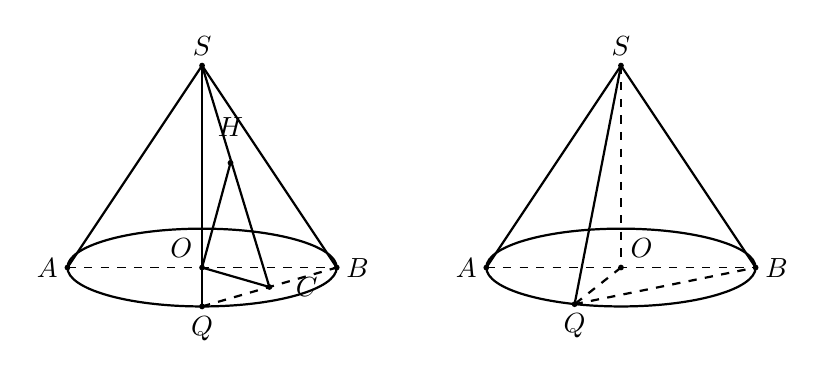
\begin{tikzpicture}[>=stealth,scale=0.95,line join=round]
  % ===== 左图 =====
  \coordinate (S)  at (0,2.7);
  \coordinate (O)  at (0,0);
  \coordinate (A)  at (-1.8,0);
  \coordinate (B)  at (1.8,0);
  \coordinate (Q)  at (0,-0.52);
  \coordinate (C)  at (0.9,-0.26);
  \coordinate (H)  at (0.38,1.40);

  \draw[thick] (0,0) ellipse (1.8 and 0.52);
  \draw[dashed] (A)--(B);
  \draw[thick] (S)--(A);
  \draw[thick] (S)--(B);
  \draw[thick,dashed] (S)--(O);
  \draw[thick,dashed] (O)--(Q);
  \draw[thick,dashed] (Q)--(B);
  \draw[thick] (S)--(Q);
  \draw[thick] (S)--(C);
  \draw[thick] (O)--(C);
  \draw[thick] (O)--(H);

  \fill (S) circle (1.1pt) node[above] {$S$};
  \fill (O) circle (1.1pt) node[above left] {$O$};
  \fill (A) circle (1.1pt) node[left] {$A$};
  \fill (B) circle (1.1pt) node[right] {$B$};
  \fill (Q) circle (1.1pt) node[below] {$Q$};
  \fill (C) circle (1.1pt) node[right=6pt] {$C$};
  \fill (H) circle (1.1pt) node[above=6pt] {$H$};

  % ===== 右图 =====
  \begin{scope}[xshift=5.6cm]
    \coordinate (S2) at (0,2.7);
    \coordinate (O2) at (0,0);
    \coordinate (A2) at (-1.8,0);
    \coordinate (B2) at (1.8,0);
    \coordinate (Q2) at (-0.62,-0.49);

    \draw[thick] (0,0) ellipse (1.8 and 0.52);
  \draw[dashed] (A2)--(B2);
    \draw[thick] (S2)--(A2);
    \draw[thick] (S2)--(B2);
    \draw[thick] (S2)--(Q2);
    \draw[thick,dashed] (S2)--(O2);
    \draw[thick,dashed] (O2)--(Q2);
    \draw[thick,dashed] (Q2)--(B2);

    \fill (S2) circle (1.1pt) node[above] {$S$};
    \fill (O2) circle (1.1pt) node[above right] {$O$};
    \fill (A2) circle (1.1pt) node[left] {$A$};
    \fill (B2) circle (1.1pt) node[right] {$B$};
    \fill (Q2) circle (1.1pt) node[below] {$Q$};
  \end{scope}
\end{tikzpicture}
